\chapter{Copy Protection Status Quo}
\label{chapter:copy_protection_status_quo}

Like introduced in \autoref{chapter:android_status_quo} there
are different goals of copy protection mechanisms starting from
preventing reverse code engineering to protect intellectual property
and reaching to hinder patching to get prohibited access.
The common denominator of those goals is the protection of
the DEX file of every app. A variety of tools do exist that
are able to transform DEX into different readable formats,
modify it and repack it again since the DEX contains
a lot of meta data for its contents (classes, methods, \ldots)
\parencite{dex}.


\section{DEX Dissassembly and Repackaging}
Generally there do exist two possible outcomes of DEX disassembling
- Java code (\code{*.java}) and Smali code (\code{*.smali}).
Since the DEX format is more or less just a different mapping of a
JAR and its containing \code{.class} files, the transition to JAR
is quite simple \parencite{dvminternals}. A tool that is able to
perform this step is ``dex2jar'' \parencite{dex2jartool}.
Along with this JAR, standard Java decompiler like ``JD-GUI''
\parencite{jdtool} can be used to produce the \code{*.java} source code.
If the \code{*.java} is supposed to change and repacked, it can
be again compiled into JAR with Oracle's ``javac'' \parencite{javactool}
followed by Googles ``dx'' tool \parencite{dxtool}
to produce the manipulated DEX.

The alternative way is the use of ``smali/baksmali'' tool
\parencite{smalitool} which is a direct assembler and disassembler
for DEX files rather than taking the Java code detour. There is also
a tool included that can convert the ODEX back to DEX.

Overall, the dissassembly of DEX is quite easy and is shown as a
concluding overview in \autoref{fig:dex_disassembly}

Therefore several countermeasures were established which are
described in the following sections.

\begin{figure}[htb]
  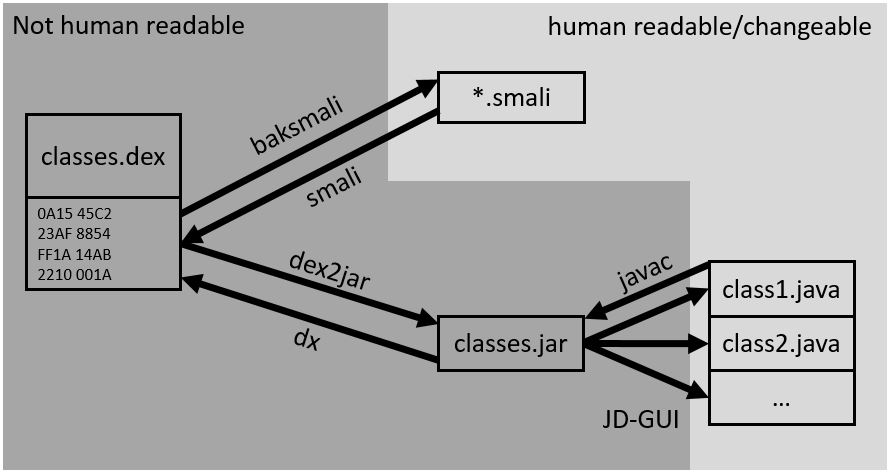
\includegraphics[width=\textwidth]{figures/dex_disassembly}
  \caption[DEX Assembly/Disassembly]{DEX Assembly/Disassembly}
  \label{fig:dex_disassembly}
\end{figure}


\section{DEX Obfuscation}
One of the most direct and effective methods of protecting source
code is obfuscation. It can be imagined like an tool-automated
additional step between the readable source code written by a human
and the compilation to the next unit, thus a transition from source
code to source code with masked functionality. An obfuscation
can be achieved with different methods which are described in
\parencite{lvl_imp}. Among other things they consist of renaming
classes, variables, functions, irreducable code insertion,
artificial parallelization, method inlining/outlining, unrolling
loops, encoding strings and so on.
The goal is to increase the complexity of code
massively by keeping its functionality. Popular obfuscation tools
are Google's ``ProGuard'' \parencite{proguardtool} which is included
in the Android build system and can be enabled easily as well as
``DexGuard'' by GuardSquare \parencite{dexguardtool}.

\section{Junk-Byte-Insertion}
Junk-Byte-Insertion's goal is to confuse static analyzing
disassembling tools. It does work for tools which are
using the ``linear sweep'' to analyze a file. That means
the tools are processing every instruction from the entrypoint
till the end without interpreting them which means that bytes can
be inserted that are never reached by executing the code
(for instance because there is an if-else- construct that is
always true) but will be processed by the tool and will break the
resulting disassembled code \parencite{lvl_imp}.

\section{Code Encryption}
